%%%%%%%%%%%%%%%%%%%%%%%%%%%%%%%%%%%%%%%%%%%%%%%%%%%%%%%%%%%%
\documentclass[xcolor=x11names,compress, handout]{beamer}

\definecolor{CoolBlack}{rgb}{0.0, 0.18, 0.39}
\definecolor{byellow}{rgb}{0.55037, 0.38821, 0.06142}
%% General document %%%%%%%%%%%%%%%%%%%%%%%%%%%%%%%%%%
\usepackage{graphicx}
\usepackage{tikz}
\usepackage{Tabbing}
\usetikzlibrary{decorations.fractals}
%%%%%%%%%%%%%%%%%%%%%%%%%%%%%%%%%%%%%%%%%%%%%%%%%%%%%%

%% Beamer Layout %%%%%%%%%%%%%%%%%%%%%%%%%%%%%%%%%%
\useoutertheme[subsection=false,shadow]{miniframes}
\useinnertheme{default}
\usefonttheme{serif}
\usepackage{palatino}
\usepackage{tabu}

% addition of color
\usepackage{xcolor}
\definecolor{dgreen}{rgb}{0.,0.6,0.}
\definecolor{RawSienna}{cmyk}{0,0.72,1,0.45}

\setbeamerfont{title like}{shape=\scshape}
\setbeamerfont{frametitle}{shape=\scshape}

\setbeamercolor*{lower separation line head}{bg=CoolBlack} 
\setbeamercolor*{normal text}{fg=black,bg=white} 
\setbeamercolor*{alerted text}{fg=dgreen} 
\setbeamercolor*{example text}{fg=black} 
\setbeamercolor*{structure}{fg=black} 
 
\setbeamercolor*{palette tertiary}{fg=black,bg=black!10} 
\setbeamercolor*{palette quaternary}{fg=black,bg=black!10} 

%\usepackage[sorting=none]{biblatex}
\usepackage{fancyvrb}
\usepackage{caption}
\usepackage{color}
\usepackage[version=3]{mhchem}
\mode<presentation>

% Links
\usepackage{hyperref}
\definecolor{links}{HTML}{003262}
\hypersetup{colorlinks,linkcolor=,urlcolor=links}

% columns
\renewcommand{\(}{\begin{columns}}
\renewcommand{\)}{\end{columns}}
\newcommand{\<}[1]{\begin{column}{#1}}
\renewcommand{\>}{\end{column}}

% adding slide numbers
\addtobeamertemplate{navigation symbols}{}{%
    \usebeamerfont{footline}%
    \usebeamercolor[fg]{footline}%
    \hspace{1em}%
    \insertframenumber/\inserttotalframenumber
}

% equation stuff
\usepackage{mathrsfs}
\usepackage[mathcal]{euscript}
\usepackage{amssymb}
\usepackage{amsthm}
\usepackage{epsfig}
\usepackage{amsmath}
%
%\bibliography{presentation}
%\setbeamertemplate{bibliography item}[text]

%%%%%%%%%%%%%%%%%%%%%%%%%%%%%%%%%%%%%%%%%%%%%%%%%%

\begin{document}

%%%%%%%%%%%%%%%%%%%%%%%%%%%%%%%%%%%%%%%%%%%%%%%%%%%%%%
%%%%%%%%%%%%%%%%%%%%%%%%%%%%%%%%%%%%%%%%%%%%%%%%%%%%%%
\begin{frame}
\title[Developments in WARP]{Developments in the GPU-accelerated WARP Monte Carlo Neutron Transport Code}
\author{\includegraphics[height=2cm]
{../bk-eps-converted-to}\\R.\ N.\ Slaybaugh and K.\ L.\ Rowland, UC Berkeley; \\R.\ M.\ Bergmann, Paul Shearer Institute}
\date{10 July 2015 \\ Ecole Polytechnique}
\titlepage
\end{frame}

% --------------------------------------------------------------
\begin{frame}[fragile]{Outline}
	\begin{itemize}
	\item{Motivation}
	\item{WARP}
	\begin{itemize}
	    \item{Ray tracing in WARP}
	    \item{Delta-tracking}
	    \item{Implementation of delta-tracking in WARP}
	\end{itemize}
	\item{Results}
	\item{Summary}
	\item{Future work}
	\end{itemize}
\end{frame}


% --------------------------------------------------------------
\section{\scshape Motivation}
\begin{frame}{Motivation}
	\begin{itemize}
	\pause
	\item{Graphics processing units (GPUs) have gradually increased in computational power from small,
	job-specific boards to programmable powerhouses}
	\pause
	\item{Compared to more common central processing units (CPUs), GPUs have higher aggregate memory
	bandwidth, much higher floating-point operations per second (FLOPS), and lower energy consumption
	per FLOP \cite{warp}}
	\pause
	\item{CPU-optimized parallel algorithms are not directly portable to GPUs}
	\pause
	\item{Particle transport codes need to be rewritten to execute efficiently on GPUs 
	\cite{warp}}
	\end{itemize}
\end{frame}


% --------------------------------------------------------------
\begin{frame}{Motivation}
	\begin{itemize}
	\pause
	\item{Most Monte Carlo neutron transport codes use ray tracing algorithms to track neutron 
	locations throughout their histories}
		\begin{itemize}
		\pause
		\item{WARP, originally developed at UC Berkeley, employs ray tracing \cite{warp}}
		\end{itemize}
	\pause
	\item{Woodcock delta-tracking is another, slightly different, method for following neutrons 
	\cite{serpent}}
		\begin{itemize}
		\pause
		\item{Has been implemented in CPU-based codes, but never before on a GPU-based code}
		\end{itemize}
	\pause
	\item{The purpose of this work is to implement and assess the performance of delta-tracking in a
	GPU-based Monte Carlo neutron transport code}
	\end{itemize}
\end{frame}


% --------------------------------------------------------------
\section{\scshape WARP}
\begin{frame}{WARP \cite{warp}}
	\begin{itemize}
	\pause
	\item{``Weaving All the Random Particles"}
	\pause
	\item{Originally developed by Dr. Ryan Bergmann}
	\pause
	\item{3D continuous-energy Monte Carlo neutron transport code developed for efficient 
	implementation of the algorithm on GPUs}
	\pause
	\item{Can calculate multiplication factors, flux tallies, fission source distributions for 
	time-independent problems}
	\pause
	\item{Run in either criticality or fixed-source mode}
	\pause
	\item{Simulates neutron transport in unrestricted arrangements of parallelpipeds, hexagonal 
	prisms, cylinders, and spheres}
	\end{itemize}
\end{frame}


% --------------------------------------------------------------
\begin{frame}{Ray Tracing in WARP \cite{warp}}
	\begin{itemize}
	\pause
	\item{WARP uses the NVIDIA OptiX ray tracing framework for geometry representation}
	\pause
	\item{OptiX is a highly-optimized, scalable framework developed for building applications on GPUs}
		\begin{itemize}
		\pause
		\item{Allows for user-written applications}
		\pause
		\item{OptiX engine composed of host-based API that defines ray tracing data structures 
		combined with a CUDA C-based programming system that handles the rays \cite{optix-man}}
		\end{itemize}
	\end{itemize}
\end{frame}


% --------------------------------------------------------------
\begin{frame}{Ray Tracing in WARP \cite{warp}}
	\pause
	\begin{itemize}
	\item{Material information updated only when sampled interaction distance greater than nearest
	surface distance}
		\begin{itemize}
		\pause
		\item{Neutron moves to boundary that will be crossed}
		\pause
		\item{Material information updated to material being entered}
		\pause
		\item{Interaction distance is resampled in new material with same direction of flight}
		\end{itemize}
	\pause
	\item{WARP uses an algorithm that uses ray tracing to determine the material being entered}
		\begin{itemize}
		\pause
		\item{All system geometric information stored in OptiX ``context"}
		\end{itemize}
	\end{itemize}
\end{frame}


% --------------------------------------------------------------
\begin{frame}{Material Query in WARP \cite{warp}}
\pause
\begin{columns}
	\column{0.475\linewidth}
	\begin{figure}[h!]
	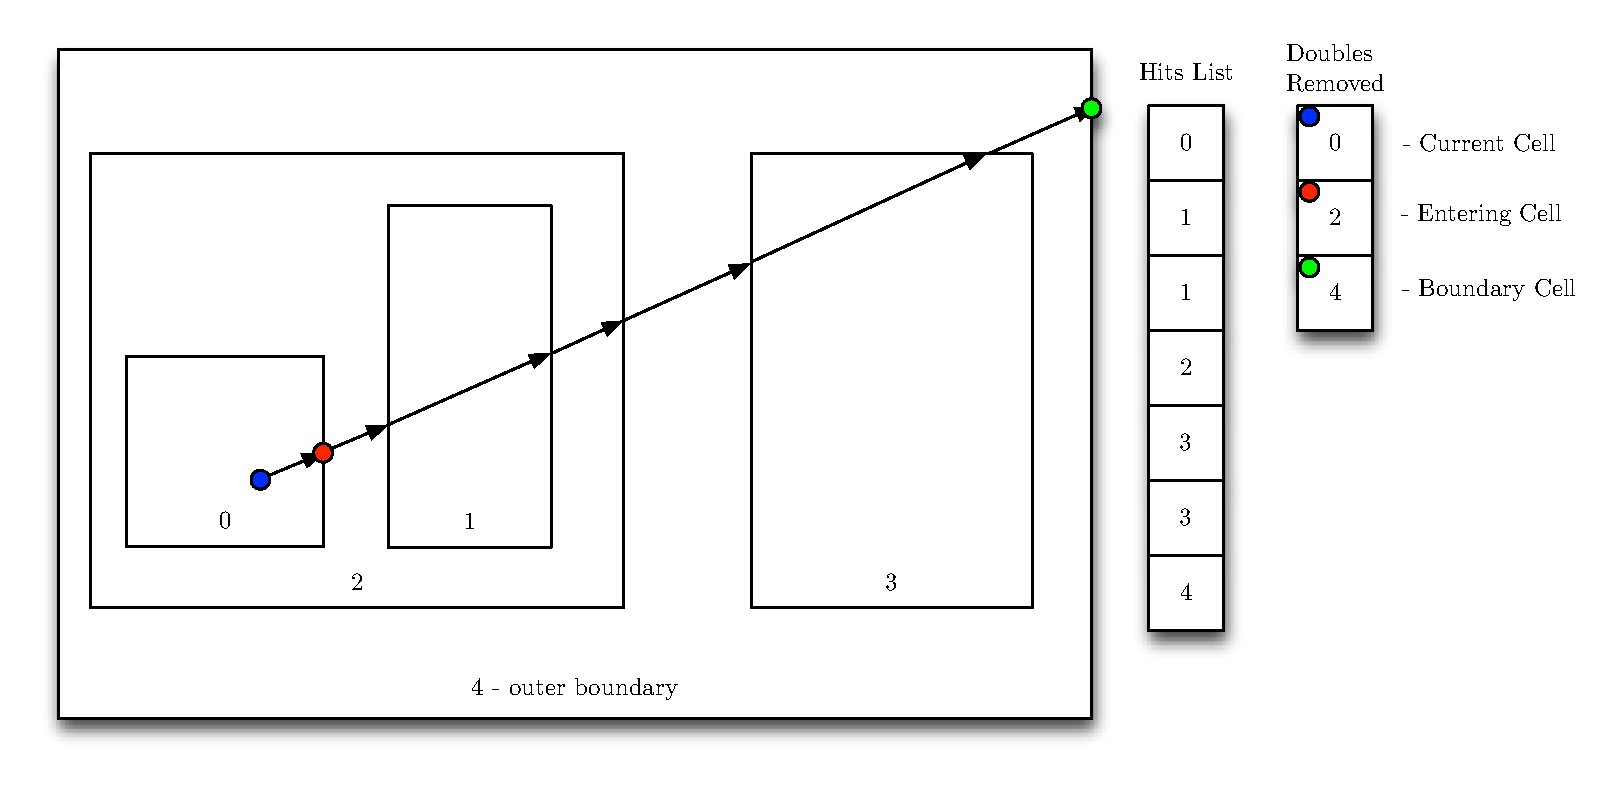
\includegraphics[width=2.5 in]{../figs/whereami}
	\caption{The point-in-polygon-like algorithm for determining the entering cell/material number by 
	using ray tracing. \label{whereami}}
	\end{figure}
	\column{0.525\linewidth}
	\begin{itemize}
	\pause
	\item{List of surface intersection generated by iteratively ray tracing along neutron direction of
	flight}
	\pause
	\item{Intersections ordered by proximity}
	\pause
	\item{Tracing stopped once ray hits predefined outer cell}
	\pause
	\item{Double entires removed from list}
	\pause
	\item{Result is list of cells in which neutron is nested}
		\begin{itemize}
		\pause
		\item{First entry is cell in which neutron is located}
		\pause
		\item{Second entry is cell that the neutron is entering}
		\end{itemize}
	\end{itemize}
\end{columns}
\end{frame}


% --------------------------------------------------------------
\begin{frame}{Issues with Ray Tracing \cite{warp}}
	\begin{itemize}
	\pause
	\item{Cell descriptions are mathematically exact, but are represented by inexact numbers}
		\begin{itemize}
		\pause
		\item{Floating-point roundoff can cause a neutron to be placed slightly behind a boundary
		instead of at the actual boundary}
		\pause
		\item{Situation preventable by using an OptiX ``scene epsilon" }
		\end{itemize}
	\pause
	\item{Scene epsilon designates the minimum distance away from the ray origin at which 
	intersection points are allowed to occur}
		\begin{itemize}
		\pause
		\item{Set by the programmer}
		\pause
		\item{Helps ensure that a trace starts after a boundary such that accurate results are
		calculated}
		\pause
		\item{Must be set to an appropriate value for the problem geometry for effective use}
		\end{itemize}
	\end{itemize}
\end{frame}


% --------------------------------------------------------------
\begin{frame}{Issues with Ray Tracing \cite{warp}}
	\begin{itemize}
	\pause
	\item{Material query inaccuracies can be caused by scene epsilon in certain geometric 
	configurations}
		\begin{itemize}
		\pause
		\item{If object thickness is less than scene epsilon, material query may only count a
		single intersection of the object}
		\pause
		\item{That object's material is then determined instead of the object being skipped}
		\pause
		\item{Can be avoided by performing material query in z-direction only}
		\pause
		\item{Currently, all objects in WARP are z-aligned prisms or spheres}
			\begin{itemize}
			\pause
			\item{Applicable to reactor geometries}
			\end{itemize}
		\end{itemize}
	\end{itemize}
\end{frame}


% --------------------------------------------------------------
\begin{frame}{Issues with Ray Tracing \cite{warp}}
	\begin{itemize}
	\pause
	\item{One other issue in using the algorithm occurs when cells have coincident surfaces}
		\begin{itemize}
		\pause
		\item{Number of cell that is intersected is undefined}
		\pause
		\item{Following trace iteration will skip the intersection of the coincident cell}
		\pause
		\item{One way to avoid this would be to ensure coincident surfaces are more than one scene
		epsilon apart}
			\begin{itemize}
			\pause
			\item{Problematic if neutron mean free path is smaller than the gap}
			\end{itemize}
		\end{itemize}
	\pause
	\item{An important consideration about WARP's geometrical representation is that the volume of a
	cell is always the spatial intersection of the volume inside of the cell with the space outside
	any cells nested inside of it}
	% a picture might help illustrate this idea
	\end{itemize}
\end{frame}


% --------------------------------------------------------------
\begin{frame}{Delta-tracking}
	\begin{itemize}
	\pause
	\item{Introduced by Woodcock in the 1960's}
	\pause
	\item{Employed in Serpent in combination with ray tracing \cite{serpent}}
	\pause
	\item{Neutron path lengths are sampled as:}
		\begin{equation*}
		\ell = \frac{-\log\xi}{\Sigma_{tot,m}(E)}
		\end{equation*}
	\pause
	\item{Not statistically valid if the neutron crosses a material boundary}
	\pause
	\item{Flight must be stopped at the boundary surface and the path length resampled with the new 
	material cross section}
	\pause
	\item{Delta-tracking effectively homogenizes cross sections so that sampled path lengths are valid
	over the entire geometry}
	\end{itemize}
\end{frame}


% --------------------------------------------------------------
\begin{frame}{Virtual Collisions and the Majorant Cross Section \cite{serpent}}
	\begin{itemize}
	\pause
	\item{``Virtual collisions" are scattering reactions that preserve neutron energy and direction}
		\pause
		\begin{itemize}
		\item{No impact on final outcome}
		\item{Any number of them can ``happen" in the random walk}
		\end{itemize}
	\pause
	\item{Materials' total cross sections can be adjusted by adding an arbitrary virtual collision 
	cross section:}
		\begin{equation*}
		\Sigma'_{tot,m}(E) = \Sigma_{tot,m}(E) + \Sigma_{0,m}(E)
		\end{equation*}
	\pause
	\item{With this, a global majorant cross section can be assigned:}
		\begin{equation*}
		\begin{aligned}
		\Sigma_{maj}(E) &= \Sigma'_{tot,1}(E) = \Sigma'_{tot,2}(E) = \ldots = \Sigma'_{tot,M}(E)\\
		& = \max\{\Sigma_{tot,1}(E), \Sigma_{tot,2}(E),\ldots, \Sigma_{tot,M}(E)\}
		\end{aligned}
		\end{equation*}
	\end{itemize}
\end{frame}


% --------------------------------------------------------------
\begin{frame}{More on the Majorant \cite{serpent}}
	\begin{equation*}
        \begin{aligned}
        \Sigma_{maj}(E) &= \Sigma'_{tot,1}(E) = \Sigma'_{tot,2}(E) = \ldots = \Sigma'_{tot,M}(E) \\
        & = \max\{\Sigma_{tot,1}(E), \Sigma_{tot,2}(E),\ldots, \Sigma_{tot,M}(E)\}
        \end{aligned}
        \end{equation*}
	\begin{itemize}
	\pause
	\item{Path lengths sampled using the global majorant are statistically valid in all materials}
	\pause
	\item{Effectively homogenizes material total cross sections and eliminates need to calculate 
	surface distances}
	\pause
	\item{One additional step is required}
		\begin{itemize}
		\pause
		\item{Rejection sampling is carried out for each collision}
		\item{Collision point accepted with probability 
		$P_{m}(E) = \Sigma_{tot,m}(E)/\Sigma_{maj}(E)$}
		\pause
		\item{If the point is rejected, the collision is considered virtual and the random walk 
		continues by sampling a new path length}
		\end{itemize}
	\end{itemize}
\end{frame}


% --------------------------------------------------------------
\begin{frame}{Advantages of Delta-tracking \cite{serpent}}
	\begin{itemize}
	\pause
	\item{Random walk can be continued over material boundaries}
	\pause
	\item{Geometry routine is reduced to determining the material at each collision point}
	\pause
	\item{Delta-tracking has been found to be faster than ray-tracing in complex geometries in the 
	CPU-based Serpent code}
	\pause
	\item{Complicated objects and surface types are easier to handle}
	\pause
	\item{Majorant cross section is independent of spatial coordinates}
	\pause
	\item{Neutrons can effectively be tracked through inhomogeneous material regions}
		\begin{itemize}
		\item{Total cross section must be known at each collision point}
		\end{itemize}
	\end{itemize}
\end{frame}


% --------------------------------------------------------------
\begin{frame}{Disadvantages of Delta-tracking \cite{serpent}}
	\begin{itemize}
	\pause
        \item{Localized heavy absorbers can result in poor efficiency of resampling loop}
                \begin{itemize}
                \pause
                \item{Absorber cross section dominates majorant}
                \item{Probability of sampling physical collision becomes low outside absorber}
                \item{Random walk is cut into many short tracks and computing time is wasted in 
		resampling}
                \end{itemize}
	\pause
	\vspace*{1 em}
	\item{Must use collision flux estimator rather than track-length estimator to calculate reaction 
	rate integrals}
		\begin{itemize}
		\pause
		\item{Poor efficiency for tallies scored in small/thin regions and in materials with low 
		collision density}
		\item{Integral flux can be underestimated by collision flux estimator}
		\item{Should not be considered a disadvantage for WARP; the code uses the collision flux 
		estimator}
		\end{itemize}
	\end{itemize}
\end{frame}


% --------------------------------------------------------------
\begin{frame}[fragile]{Implementation of Delta-tracking in WARP}
	\pause
	Calculation of the majorant cross section:
	\vspace{5 mm}
	\pause
	\begin{Verbatim}[fontsize=\footnotesize]
	for(int i = 0; i < n_materials; i++){
	    for(int j = 0; j < n_isotopes; j++){
	            num_dens = material_matrix[n_isotopes*i + j];
	            if(num_dens > 0.0){
	                t0 = xs_data_MT[n_columns*dex     + j];
	                t1 = xs_data_MT[n_columns*(dex+1) + j];
	                macro_t_total+=((t1-t0)/(e1-e0)*(this_E-e0)+t0)*num_dens;
	            }
	    }
	    if(macro_t_total > majorant){majorant = macro_t_total;}
	    macro_t_total = 0.0;
	}
	\end{Verbatim}
\end{frame}


% --------------------------------------------------------------
\begin{frame}[fragile]{Implementation of Delta-tracking in WARP}
	\pause
	Calculation of the total macroscopic cross section:
	\vspace{5 mm}
	\pause
	\begin{Verbatim}[fontsize=\footnotesize]
	for(int k=0; k < n_isotopes; k++){
	    num_dens = material_matrix[n_isotopes*this_mat + k];
	        if(num_dens > 0.0){
	            t0 = xs_data_MT[n_columns* dex    + k];
	            t1 = xs_data_MT[n_columns*(dex+1) + k];
	            macro_t_total+=((t1-t0)/(e1-e0)*(this_E-e0)+t0)*num_dens;
	        }
	}
	\end{Verbatim}
\end{frame}


% --------------------------------------------------------------
\begin{frame}[fragile]{Implementation of Delta-tracking in WARP}
	\pause
	Path length sampling:
	\vspace{2 mm}
	\pause
	\begin{Verbatim}[fontsize=\footnotesize]
	samp_dist = -logf(get_rand(&rn))/majorant;
	\end{Verbatim}
	\pause
	\vspace{2 mm}
	Boundary conditions are checked, and then rejection sampling is done:
	\pause
	\vspace{2 mm}
	\begin{Verbatim}[fontsize=\footnotesize]
	float rn1 = get_rand(&rn);
	if(rn1 > macro_t_total/majorant){this_rxn=800; isdone=0; tope=999999998;}
	else{this_rxn = 0; isdone = 0;}
	x += samp_dist * xhat;
	y += samp_dist * yhat;
	z += samp_dist * zhat;
	\end{Verbatim}
\end{frame}


% --------------------------------------------------------------
\section{\scshape Results}
\begin{frame}{Results}
	\begin{itemize}
	\pause
	\item{All runs done on an NVIDIA GeForce GTX TITAN Black graphics card}
	\pause
	\item{20 inactive cycles, 40 active cycles}
	\pause
	\item{500 000 histories}
	\pause
	\item{Vacuum boundary conditions}
	\pause
	\item{Serpent ENDF/B-VII ACE data at 300K}
	\end{itemize}
\end{frame}


% --------------------------------------------------------------
\begin{frame}{Results - Jezebel}
	\begin{itemize}
	\pause
	\item{Bare plutonium sphere, considered a standard criticality test \cite{nea1995}}
	\pause
	\item{Geometry configuration is a Pu-239 sphere with a radius of 5.1 cm}
	\pause
	\item{Ray tracing: $k_{\mathrm{eff}} = 1.027853 \pm 3.8304 \times 10^{-4}$ in 16.17 s}
	\pause
	\item{Delta-tracking: $k_{\mathrm{eff}} = 1.028038 \pm 3.3172 \times 10^{-4}$ in 16.02 s}
	\pause
	\item{Results are acceptable within statistical uncertainty}
	\end{itemize}
\end{frame}


% --------------------------------------------------------------
\begin{frame}{Results - Jezebel}
	\begin{figure}[h!]
	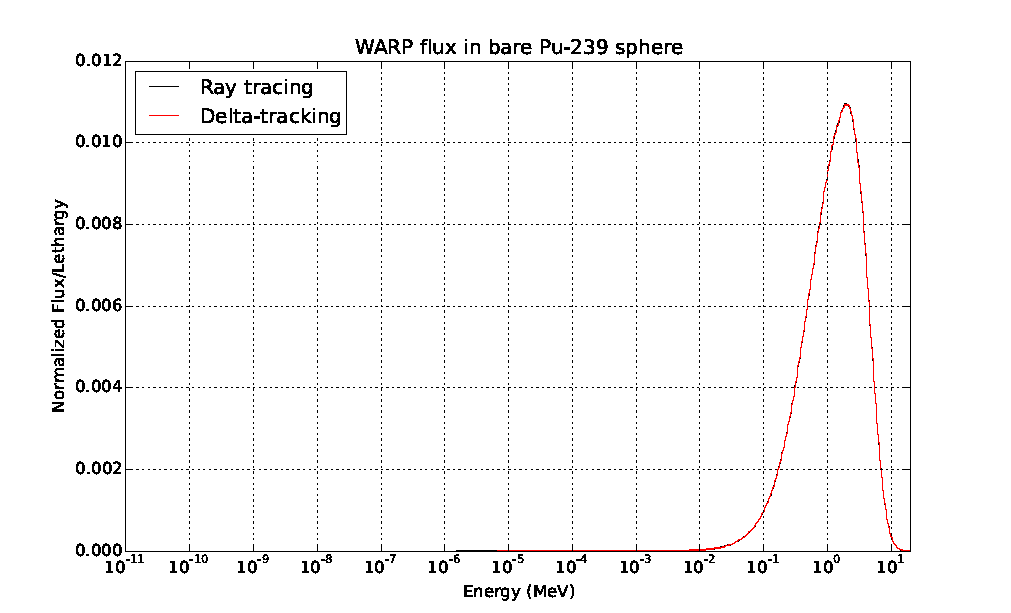
\includegraphics[width=0.9\linewidth]{../figs/godiva}
	\caption{Normalized flux spectra for the Jezebel configuration generated by both versions of WARP.
	\label{godiva}}
	\end{figure}
\end{frame}

\begin{frame}{Results - Homogenized Block}
	\begin{itemize}
	\pause
	\item{$20\times20\times20$ cm cube}
	\pause
	\item{Homogeneous mixture of 10\% $\ce{^{235}U}$ enriched $\ce{UO_2}$ and water at a 1:1 ratio}
	\pause
	\item{More complex than the Jezebel case in that its single material contains multiple isotopes}
	\pause
	\item{Ray tracing: $k_{\mathrm{eff}} = 1.213833 \pm 2.9255 \times 10^{-4}$ in 28.14 s}
	\pause
	\item{Delta-tracking: $k_{\mathrm{eff}} = 1.213983 \pm 2.1413 \times 10^{-4}$ in 30.51 s}
	\pause
	\item{Results are acceptable within statistical uncertainty}
	\end{itemize}
\end{frame}


% --------------------------------------------------------------
\begin{frame}{Results - Homogenized Block}
	\begin{figure}[h!]
	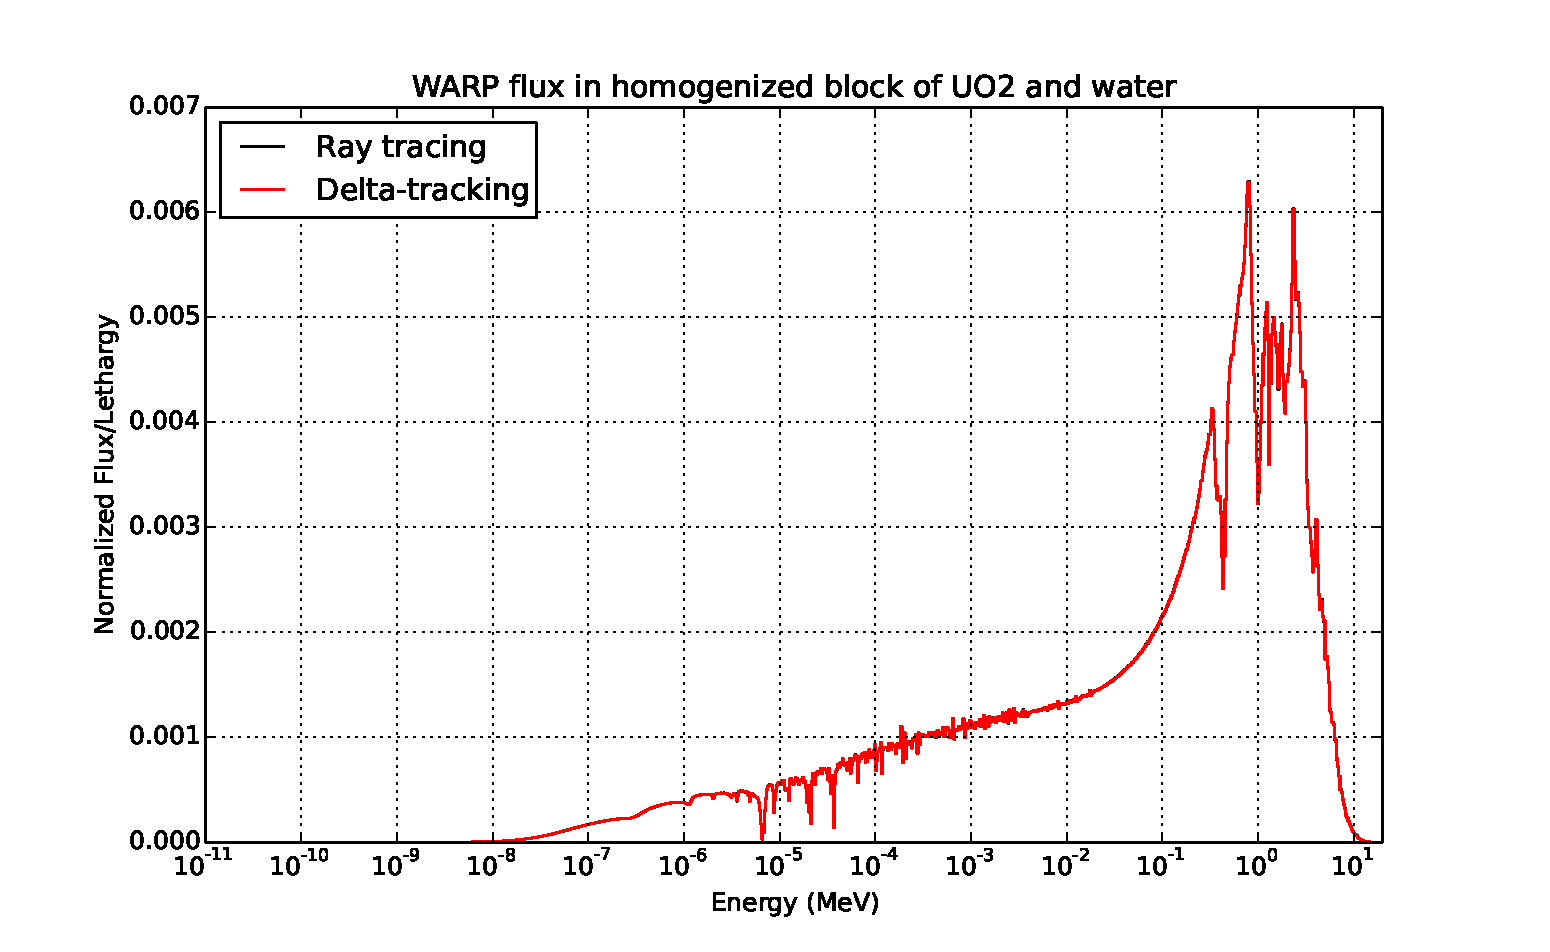
\includegraphics[width=0.9\linewidth]{../figs/homfuel}
	\caption{Normalized flux spectra for the homogenized block configuration generated by both 
	versions of WARP. \label{homfuel}}
	\end{figure}
\end{frame}


% --------------------------------------------------------------
\begin{frame}{Discussion}
	\pause
	\begin{itemize}
	\item{For homogeneous configurations, results are accurate}
	\pause
	\item{However, delta-tracking offers no great speedup in comparison to ray tracing}
		\begin{itemize}
		\pause
		\item{To be expected, no boundaries to be crossed}
		\pause
		\item{Calculations done for proof of concept and to verify correctness}
		\end{itemize}
	\pause
	\item{Likely due to extra calculations required for the majorant cross section}
	\end{itemize}
\end{frame}


% --------------------------------------------------------------
\begin{frame}{Heterogeneous Geometry Configurations}
	\begin{itemize}
	\pause
	\item{Long-term interest is in cases where delta-tracking is faster than ray tracing on CPUs}
		\begin{itemize}
		\pause
		\item{Heterogeneous geometry configurations \cite{serpent}}
		\end{itemize}
	\pause
	\item{Preliminary work has been done to implement delta-tracking for heterogeneous (multiple 
	materials, multiple cells) geometry configurations}
	\pause
	\item{At this time, the implementation is not complete}
	\end{itemize}
\end{frame}


% --------------------------------------------------------------
\section{\scshape Summary \& Future Work}
\begin{frame}{Summary}
	\begin{itemize}
	\pause
	\item{WARP is a GPU-based Monte Carlo code that uses a ray tracing algorithm}
		\begin{itemize}
		\pause
		\item{Ray tracing has advantages and disadvantages}
		\end{itemize}
	\pause
	\item{Delta-tracking method was implemented in a GPU-based code for the first time}
		\begin{itemize}
		\pause
		\item{Delta-tracking also has advantages and disadvantages}
		\end{itemize}
	\pause
	\item{Use of delta-tracking calculates accurate results for homogeneous systems}
	\pause
	\item{Extension of the method to handle heterogeneous systems is underway}
	\end{itemize}
\end{frame}


% --------------------------------------------------------------
\begin{frame}{Future Work}
	\begin{itemize}
	\pause
	\item{Investigate heterogeneous geometry configurations}
	\pause
	\item{Retest delta-tracking if WARP moves to universe-based geometry similar to MCNP and Serpent}
	\pause
	\item{Delta-tracking may prove useful in a future version of WARP that has been extended for use 
	on CPU-based coprocessors}
	\end{itemize}
\end{frame}


% --------------------------------------------------------------
\begin{frame}{Acknowledgements}
\begin{center}
This material is based upon work supported under an Integrated University Program Graduate Fellowship.

\vspace{10 mm}
This work was partially supported by the Department of Energy National Nuclear Security Administration 
under Award Number(s) DE-NA0000979: The National Science and Security Consortium (NSSC), 
http://nssc.berkeley.edu/.
\end{center}
\begin{figure}
	\begin{minipage}{.45\textwidth}
	\centering
	
\includegraphics[width=0.9\linewidth]{../figs/DOE-IUP_Logo}
	\end{minipage}
	\begin{minipage}{.45\textwidth}
	\centering
	
\includegraphics[width=0.9\linewidth]{../figs/NSSC_newLogo_large}
	\end{minipage}
\end{figure}
\end{frame}


% --------------------------------------------------------------
\begin{frame}[fragile]
  \frametitle{Questions?}
  \begin{center}
  \includegraphics[height=3in,clip]{../questions-comic}  
  \end{center}
\end{frame}

% --------------------------------------------------------------
%\begin{frame}[plain,noframenumbering]{References}
%	\printbibliography
%\end{frame}

% --------------------------------------------------------------
\begin{frame}[plain,noframenumbering]{References}
	\bibliographystyle{unsrt}
	\bibliography{gpu-warp}
\end{frame}


%% --------------------------------------------------------------
%\begin{frame}[plain,noframenumbering]{Results - Pin Cell}
%	\begin{itemize}
%	\item{Bare $\ce{UO_2}$ cylinder encased in a block of water}
%	\item{Pin has 1 cm diameter and 40 cm length}
%	\item{Water block has dimensions $10\times10\times50$ cm}
%	\item{Two materials, each with multiple isotopes, and two cells}
%	\item{Ray tracing: $k_{\mathrm{eff}} = 3.798339 \times 10^{-1} \pm 6.3999 \times 10^{-4}$ in 
%	3.66683 min}
%	\item{Delta-tracking: $k_{\mathrm{eff}} = 3.822616 \times 10^{-1} \pm 4.9758 \times 10^{-4}$ in 
%	3.703 min}
%	\end{itemize}
%\end{frame}
%
%
%% --------------------------------------------------------------
%\begin{frame}[plain,noframenumbering]{Results - Pin Cell (continued)}
%	\begin{figure}[h!]
%	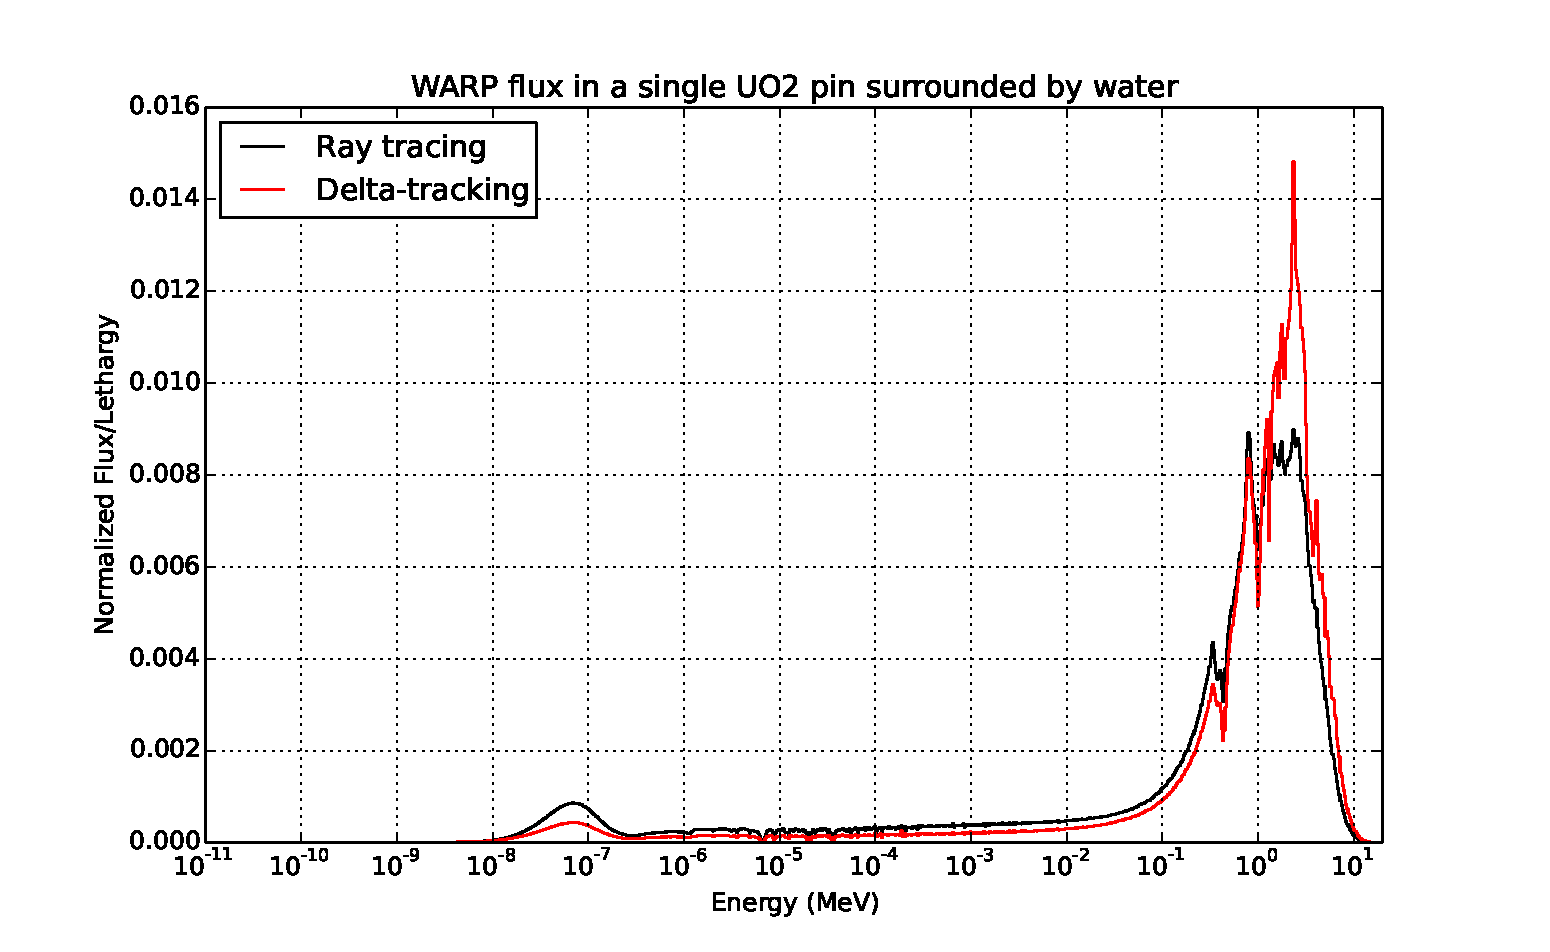
\includegraphics[width=0.9\linewidth]{../figs/pincell-fuel}
%	\caption{Normalized flux spectra for the \textbf{$\ce{UO_2}$ cylinder} in the pin cell 
%	configuration generated by both versions of WARP. \label{pincell-fuel}}
%	\end{figure}
%\end{frame}
%
%
%% --------------------------------------------------------------
%\begin{frame}[plain,noframenumbering]{Results - Pin Cell (continued)}
%	\begin{figure}[h!]
%	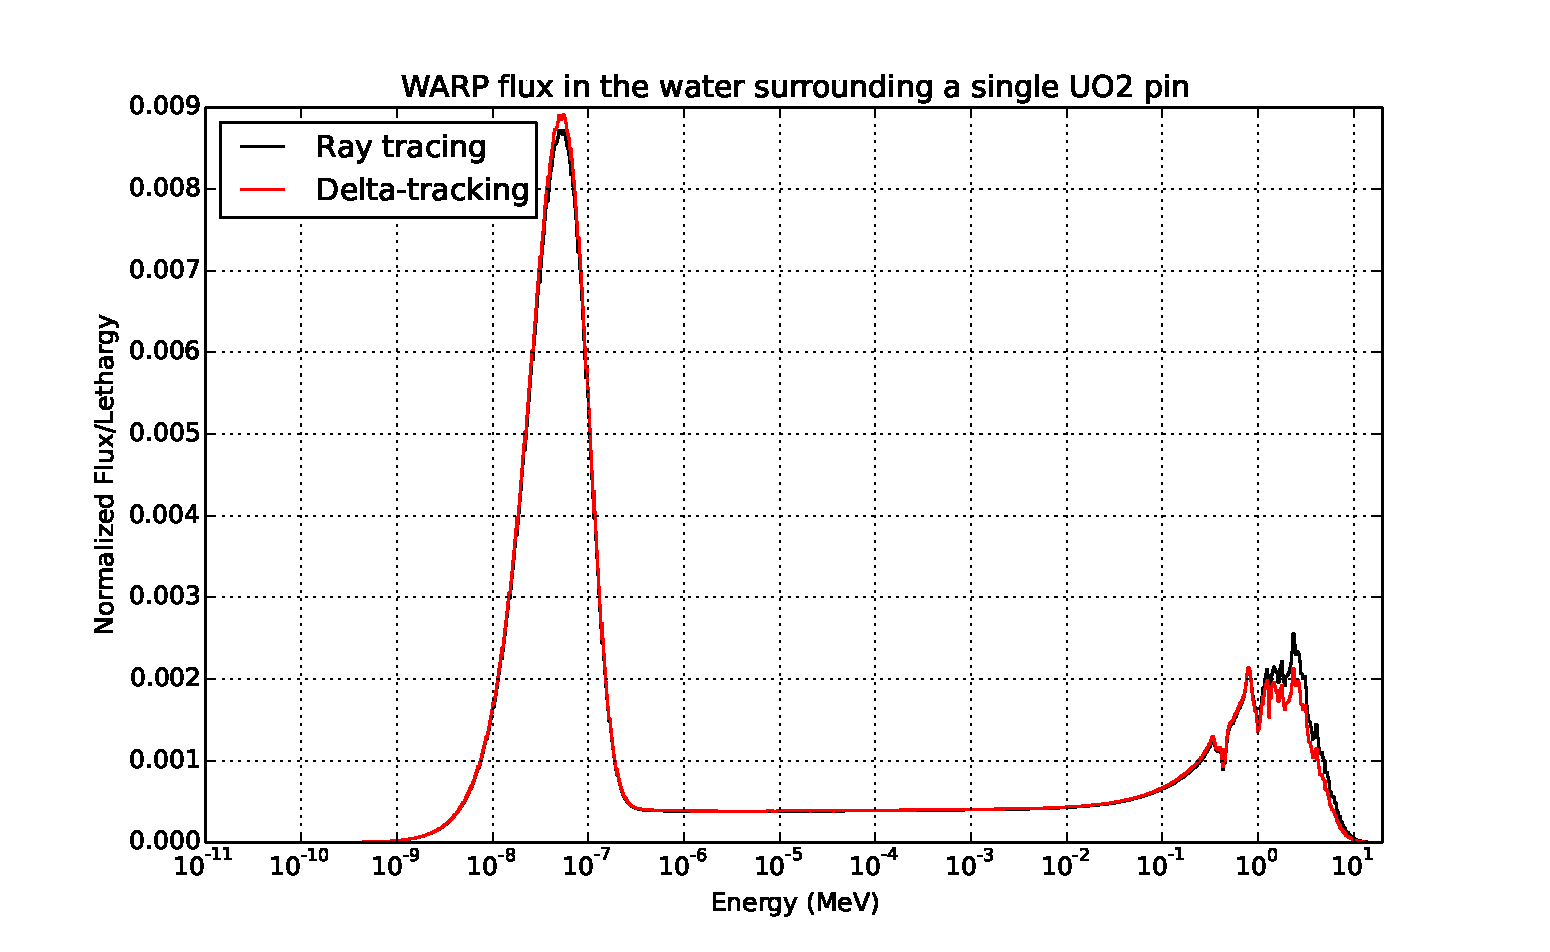
\includegraphics[width=0.9\linewidth]{../figs/pincell-water}
%	\caption{Normalized flux spectra for the \textbf{water} block in the pin cell configuration 
%	generated by both versions of WARP. \label{pincell-water}}
%	\end{figure}
%\end{frame}
%
%
%% --------------------------------------------------------------
%\begin{frame}[plain,noframenumbering]{Results - Hex Assembly}
%	\begin{itemize}
%	\item{631 $\ce{UO_2}$ cylinders arranged in a hexagonal lattice surrounded by an 
%	$84\times84\times84$ cm cube of water}
%	\item{Material compositions and cylinder dimensions identical to those in pin cell case}
%	\item{Large number of objects intended to highlight effect of introducing many geometric objects
%	into a problem}
%	\item{Ray tracing: $k_{\mathrm{eff}} = 1.445201 \pm 2.3456 \times 10^{-4}$ in 4.36917 min}
%	\item{Delta-tracking: $k_{\mathrm{eff}} = 1.415779 \pm 1.9934 \times 10^{-4}$ in 4.57683 min}
%	\end{itemize}
%\end{frame}
%
%
%% --------------------------------------------------------------
%\begin{frame}[plain,noframenumbering]{Results - Hex Assembly (continued)}
%	\begin{figure}[h!]
%	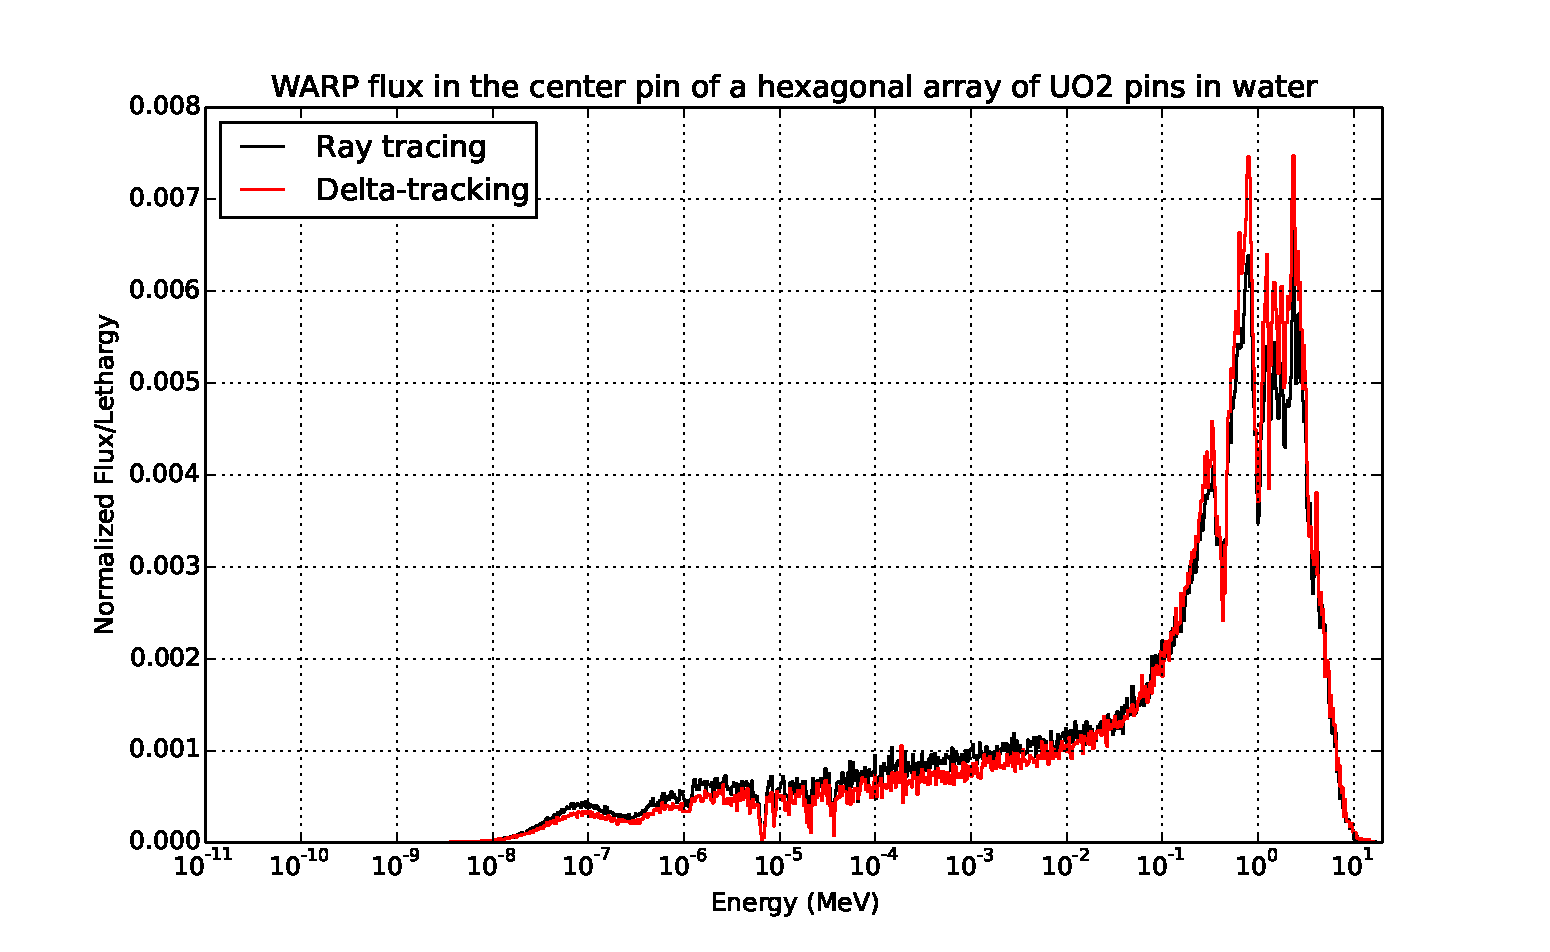
\includegraphics[width=0.9\linewidth]{../figs/assembly-centerpin}
%	\caption{Normalized flux spectra for the \textbf{center pin} of a hexagonal array of $\ce{UO_2}$ 
%	pins in water generated by both versions of WARP. \label{assembly-centerpin}}
%	\end{figure}
%\end{frame}
%
%\begin{frame}[plain,noframenumbering]{Results - Hex Assembly (continued)}
%	\begin{figure}[h!]
%	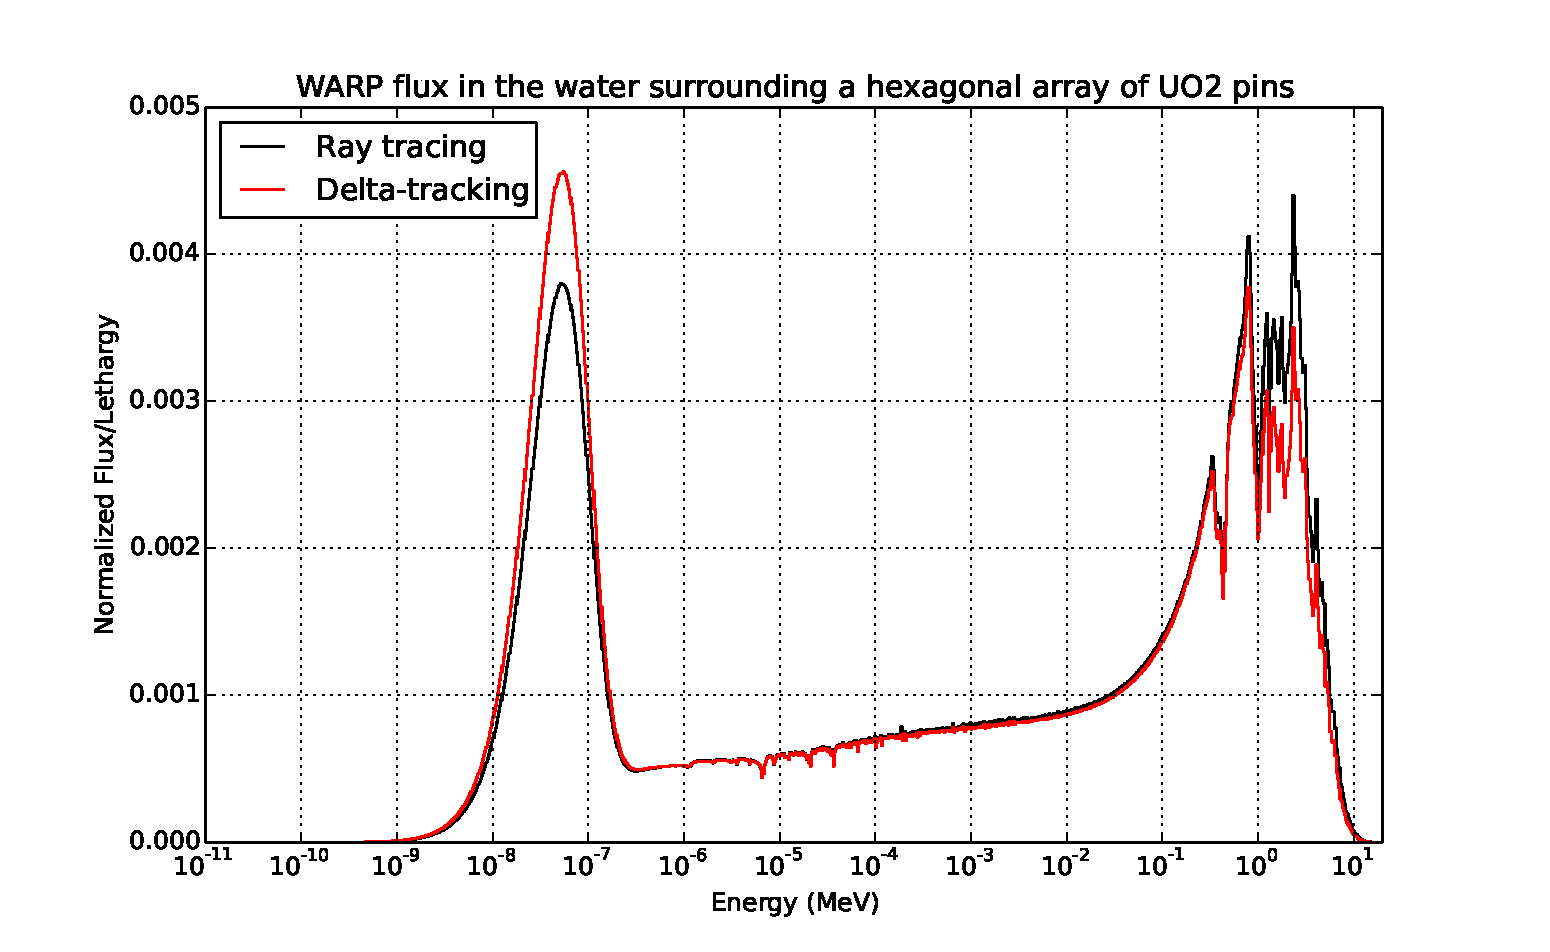
\includegraphics[width=0.9\linewidth]{../figs/assembly-water}
%	\caption{Normalized flux spectra for the \textbf{water} surrounding a hexagonal array of 
%	$\ce{UO_2}$ pins generated by both versions of WARP. \label{assembly-water}}
%	\end{figure}
%\end{frame}
\end{document}
